\documentclass[12pt,oneside]{book}

\usepackage[foundations, arithmetic]{../../lib/tex/naproche}
\usepackage{../../lib/tex/libraries}
\usepackage{graphicx}
\usepackage{float}
\usepackage{caption}
\usepackage[nobottomtitles]{titlesec}

\setlength{\headheight}{15pt}


\title{Arithmetic}
\author{Marcel Schütz}
\date{2022}

\begin{document}
  \maketitle

  \tableofcontents

  \paragraph*{}
  \begin{figure}[H]
    \centering
    \fbox{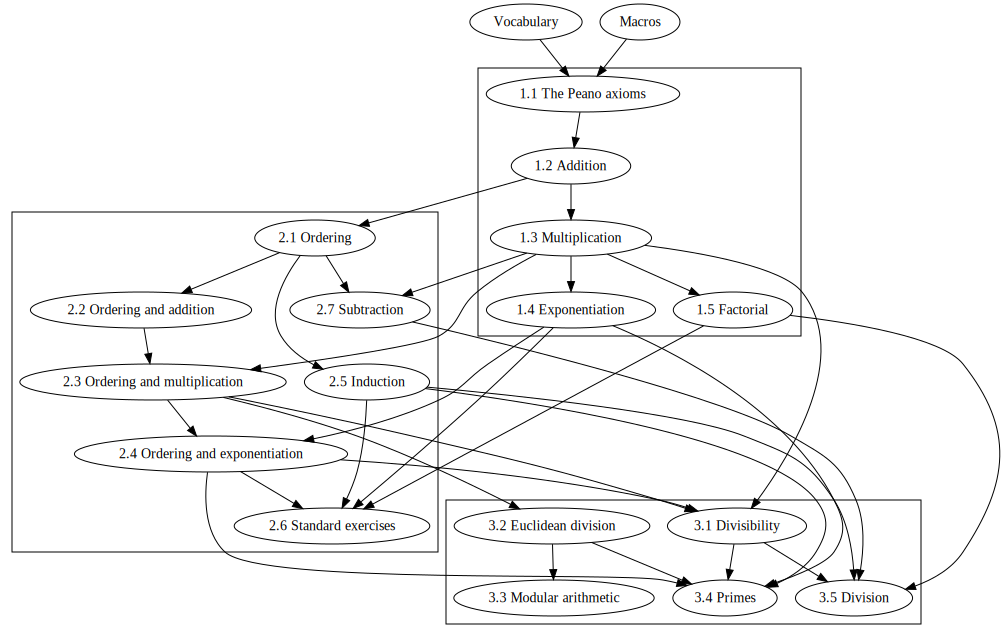
\includegraphics[width=0.9\textwidth]{./dependency-graph/graph.png}}
    \caption*{Interdependencies of the chapters}
  \end{figure}


  \section*{Introduction}

  This is a library providing basic notions of natural numbers arithmetic.
  It introduces the natural numbers on the basis of the Peano
  Axioms (\cref{chapter:natural-numbers}) and uses Dedekind's Recursion Theorem
  (\cref{chapter:recursion}) to define common arithmetical operations on them.
  A first example of such operations is given by addition
  (\cref{chapter:addition}), on the basis of which the standard ordering on the
  natural numbers is defined (\cref{chapter:ordering}) and also a (partial)
  subtraction operation (\cref{chapter:subtraction}).
  Another example of arithmetical operations is provided by multiplication
  (\cref{chapter:multiplication}) which is further used to define the notions of
  divisibility (\cref{chapter:divisibility}) and Euclidean division
  (\cref{chapter:euclidean-division}).
  Moreover, an exponentiation operation is defined
  (\cref{chapter:exponentiation}) and the notion of prime numbers is introduced
  (\cref{chapter:primes}).
  Furthermore, a chapter on cardinality (\cref{chapter:cardinality}) provides
  notions concerning finite, countable and uncountable sets.


  \paragraph*{Usage.}
  At the very beginning of each chapter you can find the name of its source
  file, e.g. \path{arithmetic/sections/01_natural-numbers.ftl.tex} for
  \cref{chapter:natural-numbers}.
  This filename can be used to import the chapter via \Naproche's
  \texttt{readtex} instruction to another ForTheL text, e.g.:

  \begin{center}
    \verb`[readtex \path{arithmetic/sections/01_natural-numbers.ftl.tex}]`
  \end{center}

  \paragraph*{Checking times.}
  The checking times for each of the chapters may vary from computer to
  computer, but on mid-range hardware they are likely to be similar to those
  given in table below:

  \begin{center}
    \begin{tabular}{c|c|c}

      & \multicolumn{2}{c}{\textbf{Checking time}}
      \\
      \textbf{Chapter}
      & \textbf{without dependencies}     & \textbf{with dependencies}
      \\ \hline
      \ref{chapter:natural-numbers}
      & 00:15 min                         & 06:55 min
      \\
      \ref{chapter:recursion}
      & 02:25 min                         & 09:20 min
      \\
      \ref{chapter:addition}
      & 01:55 min                         & 11:15 min
      \\
      \ref{chapter:ordering}
      & 03:05 min                         & 14:35 min
      \\
      \ref{chapter:subtraction}
      & 00:50 min                         & 15:25 min
      \\
      \ref{chapter:multiplication}
      & 05:35 min                         & 21:00 min
      \\
      \ref{chapter:divisibility}
      & 00:45 min                         & 21:45 min
      \\
      \ref{chapter:euclidean-division}
      & 04:00 min                         & 25:00 min
      \\
      \ref{chapter:exponentiation}
      & 07:55 min                         & 28:55 min
      \\
      \ref{chapter:primes}
      & 03:30 min                         & 29:15 min
      \\
      \ref{chapter:cardinality}
      & 07:50 min                         & 24:50 min
    \end{tabular}
  \end{center}


  \subfile{sections/01_natural-numbers.ftl.tex}
  \subfile{sections/02_recursion.ftl.tex}
  \subfile{sections/03_addition.ftl.tex}
  \subfile{sections/04_ordering.ftl.tex}
  \subfile{sections/05_subtraction.ftl.tex}
  \subfile{sections/06_multiplication.ftl.tex}
  \subfile{sections/07_divisibility.ftl.tex}
  \subfile{sections/08_euclidean-division.ftl.tex}
  \subfile{sections/09_exponentiation.ftl.tex}
  \subfile{sections/10_primes.ftl.tex}
  \subfile{sections/11_cardinality.ftl.tex}
\end{document}
